\documentclass[11pt]{article}
\usepackage[margin=25mm]{geometry}
\usepackage{lmodern}
\usepackage[T1]{fontenc}
\usepackage[utf8]{inputenc}
\renewcommand{\ttdefault}{lmtt}
\usepackage{amsmath,amssymb,amsthm,mathtools,booktabs,graphicx,microtype}
\usepackage{xcolor}
\usepackage[hidelinks]{hyperref}
\newtheorem{theorem}{Theorem}
\newtheorem{proposition}[theorem]{Proposition}
\newtheorem{lemma}[theorem]{Lemma}
\newtheorem{corollary}[theorem]{Corollary}
\newcommand{\KL}{D_{\mathrm{KL}}}
\newcommand{\HH}{\mathcal H}
\newcommand{\delt}{\delta}
\newcommand{\ee}{\varepsilon}
\newcommand{\Ckl}{\mathcal K}
\newcommand{\op}{\mathrm{op}}
\newcommand{\dist}{\operatorname{dist}}
\newcommand{\rank}{\operatorname{rank}}
\newcommand{\ds}{\displaystyle}
\newcommand{\given}{\,\middle|\,}
\DeclareMathOperator{\TV}{TV}
\newif\ifstandalonesupp

\standalonesupptrue
\title{Mathematical Supplement\\[3pt]\large When Nearly Rank-One Predictions Require Large Sequential Models}
\author{Vashista Nobaub\\Datar Consulting}
\date{November 2026}
\begin{document}
\maketitle
\noindent This supplement presents the complete argument for the simultaneous lower bounds on a single proper binary trace law, the finite-state exponent, and the transfer to measured sequence probabilities.
\begin{theorem}[Simultaneous separation, restated]\label{th:joint}
For fixed $k\ge1$ and $M>0$, the normalized mixture defined in the following section satisfies $\sigma_2(H_{p_m})\to0$ and $\liminf_m\delta_k(H_{p_m})\ge 1/(2\sqrt{\binom{2k}{k}})$. At rank one the limit equals $1/2$. The least positive-state budget for any vanishing KL tolerance has logarithmic growth exponent one in the rare-word length $L=m2^m$.
\end{theorem}
\begin{theorem}[Sharp tradeoff, restated]\label{th:frontier}
If $N_m\ge k+2$ eventually and $\log N_m/\log L\to\rho\in[0,1]$, then the optimal excess log-loss on the lexicographic family tends to $M(1-\rho)\log2$.
\end{theorem}
\begin{figure}[ht]\centering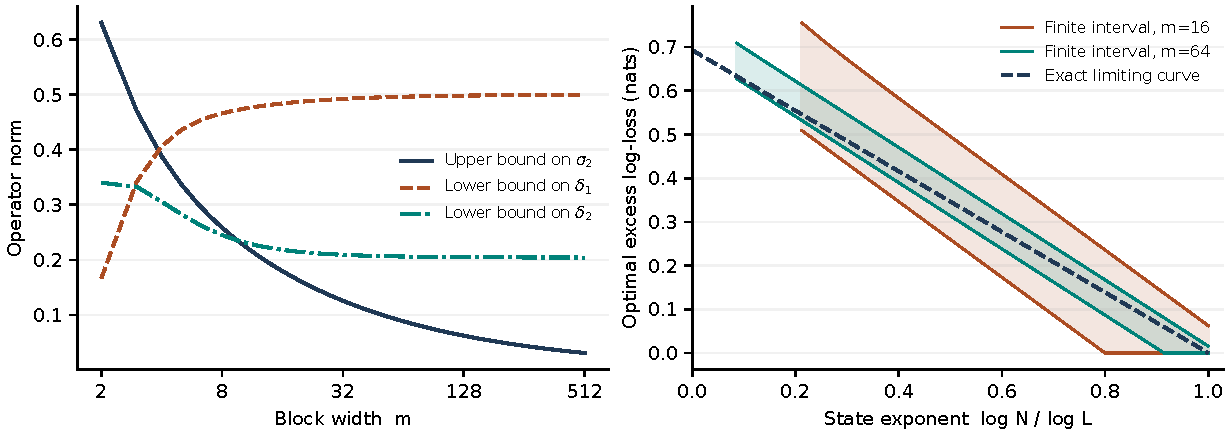
\includegraphics[width=\linewidth]{figures/joint.pdf}
\caption{Finite operator and log-loss bounds for the common law.}\label{fig:joint}\end{figure}
\appendix
\section{Finite operator witnesses}\label{app:op}
The proofs below use the notation of the main text. For an independent reading, \(k\ge1\) is a rank budget, \(m\ge2\), \(K=2^m\), \(L=mK>M>0\), \(r=1-1/m\), \(q=1-r^2\), \(\eta=M/L\), and \(t=(1-\eta)/(1+r)\). All shifts act on counting-measure word space, with inner product linear in the second argument. The direction of a concatenation matters.

\subsection{Decomposing the waiting component}
For \(0\le j\le k\), define \(z_j=\sqrt q\sum_{n\ge0}r^n e_{a^n b^j}\). These unit vectors have disjoint supports. Let \(f(a^n b^k)=qr^n\) and \(f=0\) elsewhere. Thus \(h=f/(1+r)\) is normalized. Sorting the possible cuts before or inside the terminal block gives
\[
 H_f=z_0z_k^*+\sqrt q\sum_{j=0}^{k-1}z_{k-j}e_{b^j}^* .
 \tag{S1}
\]
Indeed a cut in the waiting prefix leaves \(a^i b^k\) on the right, contributing \(qr^{n+i}\) at row \(a^n\). A cut later leaves exactly \(j<k\) copies of \(b\) on the right, contributing \(qr^n\) at row \(a^n b^{k-j}\). The input vectors \((z_k,e_{\ee},\ldots,e_{b^{k-1}})\) are orthonormal, as are the output vectors. Equation (S1) is a singular decomposition with spectrum \(1,\sqrt q,\ldots,\sqrt q\). For any word \(w\), the operator \(H_{\mathbf 1_w}\) maps a suffix basis vector to its complementary prefix, and all other vectors to zero. It is a partial permutation of norm one.

\subsection{An annihilating polynomial respects every continuation}
For a bounded competitor \(G=H_g\) of rank \(s\le k\), let \(V\) be its column space. Write \(c_v[u]=g(uv)\). The right shift \(R_b e_u=e_{ub}\) is isometric, and \(R_b^*c_v=c_{bv}\); hence its restriction \(B=R_b^*|_V\) is a contraction. Multiply its characteristic polynomial by \(z^{k-s}\) and write the result as \(P(z)=z^k+\sum_{j<k}d_jz^j\). Its roots lie in the closed unit disk, so \(|d_j|\le\binom{k}{j}\) and
\[
 S:=\sum_{j<k}|d_j|^2\le \binom{2k}{k}-1.
\]
This also covers \(G=0\) using \(P(z)=z^k\). Apply \(P(B)c_\ee=0\), followed by \(n\) backward right shifts for \(a\). It follows that \(c_{a^n b^k}+\sum_{j<k}d_j c_{a^n b^j}=0\) for each \(n\). Multiplying by \(\sqrt q\,r^n\) and summing in the Hilbert space shows that \(Gx=0\) for \(x=z_k+\sum_{j<k}d_jz_j\). By (S1),
\[
 \|x\|^2=1+S,\qquad \|H_f x\|^2=1+q^2S .
\]
Their squared ratio decreases with \(S\). This gives the structural floor \(\sqrt{(1+(C_k-1)q^2)/C_k}\) for the unnormalized \(H_f\). The argument applies over either field.

For bounded operators, both \(\sigma_2\) (on the compact operators here) and distance to a fixed nonempty subset are 1-Lipschitz in operator norm. Positive scaling commutes with both functions because the structured comparison set is a cone. Now \(H_{p_m}=tH_f+\eta H_{\mathbf1_{w_m}}\), so (S1), the structural floor and the partial permutation estimate prove the finite spectral bounds in Theorem~\ref{th:joint}. In particular, \(\|H_{p_m}\|\to1/2\): the small second singular value is meaningful also relative to the leading one.

\subsection{A sharp limiting constant at rank one}
A nonzero rank-one word-Hankel has a scalar realization \(g(w)=c\prod_{i}x_{w_i}\), with \(c\ne0\). This follows by restricting the backward shifts to its one-dimensional column space; the empty column cannot vanish for a nonzero series. Boundedness forces \(|x_a|^2+|x_b|^2<1\), since its empty column has finite square norm. The row space is spanned by the conjugate of the product sequence. Let \(P\) project onto it and write \(u=|x_a|\), \(v=|x_b|\). For \(k=1\) the absolute normalized overlap of this row with \(z_1\) is at most
\[
 \sqrt q\,\frac{v\sqrt{1-u^2-v^2}}{1-ru}
 \le\sqrt q\,\frac{1-u^2}{2(1-ru)}
 \le\sqrt q .
\]
The first inequality after the fraction maximizes over \(v\); the last uses \(1-u^2\le2(1-u)\le2(1-ru)\). Since \(G(I-P)=0\) and \(H_f^*z_0=z_1\), we have \(\|H_f-G\|\ge\|(I-P)z_1\|\ge\sqrt{1-q}=r\). The zero competitor has error one. Thus \(tr-\eta\le\delta_1(H_{p_m})\le t+\eta\), with both sides tending to \(1/2\). This sharper bound is used in Figure~\ref{fig:joint}.

\paragraph{Sharper constants inherited at other budgets.}
If the boundary limit \(E_{k-1}^{\mathbb F}\) for the unnormalized waiting family is taken from Chapter 1 of \cite{draga}, the same Lipschitz argument gives \(\lim_m\delta_k^{\mathbb F}(H_{p_m})=E_{k-1}^{\mathbb F}/2\). Here \(E_j^{\mathbb F}\) is the distance of \(z^j\) in scalar \(H^2\) to coefficient series of Hankel rank at most \(j\). In particular the resulting limits at budgets two and three are \(\sqrt3/4\) and \(3/8\). The elementary bound above suffices for the simultaneous-separation theorem at every fixed budget. This distinguishes what the present proof establishes independently from the sharper result it inherits.

\section{The positive-state obstruction}\label{app:kl}
For each binary length-\(m\) block \(B\), let \(\psi(B)=\|T_B\|_{\infty\to\infty}\). Since all entries are nonnegative, it is the maximum row sum. With \(T=T_a+T_b\) substochastic,
\[
 \sum_{B\in\{a,b\}^m}\psi(B)\le\sum_{i=1}^N(T^m\mathbf1)_i\le N.
\]
Let \(w=B_1\cdots B_K\) use each block once. The initial distribution has unit \(\ell^1\) norm and \(\|\tau\|_\infty\le1\), whence
\[
 Q(w)\le\prod_{j=1}^K\psi(B_j)
       \le\left(\frac{1}{K}\sum_{j=1}^K\psi(B_j)\right)^K
       \le (N/K)^K .
\]
The middle inequality also holds when some factors vanish. Distinctness of the blocks matters; the argument cannot count \(K\) copies of a single block as distinct resources.

\paragraph{Costs of a rare event.}
For any law \(P\), projecting onto \(\{w\}\) and its complement gives \(\KL(P\Vert Q)\ge d(P(w)\Vert Q(w))\), where \(d\) is binary KL. This is the log-sum inequality applied to the complement. If \(P(w)=\eta\), the weaker but explicit form \(\KL(P\Vert Q)\ge-\eta\log Q(w)-h_2(\eta)\) follows by dropping \(-(1-\eta)\log(1-Q(w))\ge0\). Our word contains \(ba\) for \(m\ge2\), so \(h(w_m)=0\) and \(p_m(w_m)=\eta\). Substituting the cap and \(\eta K=M/m\) proves the KL inequality, uniformly in \(N\). A negative right-hand side can always be replaced by zero.

\paragraph{Finite state cost and exponent.}
Every budget with \(\Ckl_N(p_m)\le\epsilon\) satisfies
\[
 N\ge K\exp\!\left[-\frac mM\{\epsilon+h_2(M/L)\}\right].
 \tag{S2}
\]
The bound survives taking an infimum over controllers. The waiting law is generated by \(k+1\) states: the initial state loops on \(a\) with probability \(r\), enters the \(b\)-chain with probability \(1-r\), and stops after exactly \(k\) copies of \(b\). A deterministic path with \(L+1\) states emits \(w_m\) and stops. An initial distribution on the disjoint union realizes their mixture with \(L+k+2\) states. Since \(\log L=m\log2+\log m\), (S2) and this exact construction prove the exponent-one limit for every vanishing error tolerance. A fixed multiple of \(L\) as a necessary state count would be stronger than this exponent. The proof leaves the subpolynomial factor undetermined.

\paragraph{What happens to the mean?}
The source mean is exactly \((1-\eta)(k+r/(1-r))+M\). Holding \(M\) fixed bounds the exceptional branch's contribution to the mean. It does not bound the mean of the background when \(r\uparrow1\). Changing the mixture background to an empty-word atom would restore a bounded mean but remove the present structured operator witness.

\section{Matching the intermediate state budgets}\label{app:upper}
Partition the lexicographically ordered $m$-blocks into $G=2^\ell$ contiguous groups by their common $\ell$-bit prefix. Each group contains $D=2^{m-\ell}$ blocks. A controller state $(g,j)$ holds the current group and position $j\in\{1,\ldots,m\}$ within its block. When $j\le\ell$ the controller emits bit $j$ of the binary group index. At later positions it chooses a fair bit. It next increments $j$; after position $m$ it stays in the same group with probability $1-1/D$ or advances with probability $1/D$. Advancing past the last group enters one terminal state. This is a time-homogeneous proper generator: each group finishes almost surely, and there are finitely many groups. It has $mG+1$ states and does not receive an external position counter.

One particular trajectory emits the required suffix bits and stays exactly $D$ blocks in each group. Its probability under this generator $U_\ell$ is
\[
 2^{-(m-\ell)K}\left[D^{-1}(1-D^{-1})^{D-1}\right]^G .
\]
For $D=1$ the bracket equals one. For $D>1$, $-(D-1)\log(1-1/D)\le1$ by $\log(1+x)\le x$. Hence
\[
 -\log U_\ell(w_m)\le (m-\ell)K\log 2 + G(\log D+1).
\]
An initial choice between the waiting controller and $U_\ell$ in proportions $1-\eta,\eta$ uses $k+2+mG$ states. On the background support its law dominates $(1-\eta)h$ pointwise. Its contribution to $\KL(p_m\Vert Q)$ there is nonpositive; at $w_m$ it is at most $-\eta\log U_\ell(w_m)$. Since $\eta G=M/(mD)$ and $\log D+1\le D$, the asserted finite upper bound follows.

For $\rho>0$ choose $\ell=\min\{m,\lfloor\log_2((N_m-k-2)/m)\rfloor\}$, which is nonnegative for all sufficiently large $m$. Then $\ell/m\to\rho$. The upper construction and the finite lower bound prove Theorem~\ref{th:frontier}. For $\rho=0$, one can avoid spending $m$ position states. Choose the waiting controller or a single state emitting independent fair letters with stop probability $1/(L+1)$. The latter assigns $w_m$ probability $2^{-L}(L/(L+1))^L/(L+1)$. The resulting $k+2$ state mixture has divergence at most $M\log2+(M/L)(\log(L+1)+1)$, while the lower bound tends to $M\log2$. This proves the endpoint. At $\rho=1$ the first construction gives vanishing divergence even for budgets below $L$ having the same exponent.

As a consequence, for fixed $0<e<M\log2$, the least state budget for $\Ckl_N(p_m)\le e$ has exponent $1-e/(M\log2)$. Indeed (S2) supplies the lower exponent. For any larger exponent strictly less than one, the matching upper limit is strictly below $e$; take the infimum over such exponents. This tradeoff controls total excess log-loss, not log-loss per emitted action.

\section{Transfer to a measured trace probability}\label{app:transfer}
For \(0<p<1\) and \(0<c<p\), the derivative of \(d(p\Vert x)\) with respect to \(x\) is \((x-p)/(x(1-x))<0\) on \(x<p\). This proves the binary event bound after substituting the largest allowed \(x=c\); the complementary case allows \(x=p\). Endpoint conventions follow by continuity. A verified interval \(P(w)\in[p_-,p_+]\) gives the same bound evaluated at \(p_-\) if \(p_->c\), since \(d(p\Vert c)\) increases for \(p>c\). Our empirical evaluations are ordinary floating-point measurements of the exported model; we do not prove forward error bounds for quantized inference.

For a single state, write its stop probability as \(s\) and its conditional letter probabilities as \(u,1-u\). For a balanced length-\(L\) word,
\(Q(w)=s(1-s)^L[u(1-u)]^{L/2}\).
The maximum is attained at \(s=1/(L+1),u=1/2\). This proves the sharp scalar cap, including its termination factor. For example the cap for the two-action plan \(ab\) is \(1/27\), while for a length-64 word listing all four-bit blocks the general four-state cap is \(2^{-32}\). A failure to cross a cap provides no upper bound on the best attainable KL.

\subsection{A finite Hankel check on an observed policy}
A controlled horizon \(T\) defines a different law \(P^{(T)}\): use the three-token policy until it stops or has emitted \(T\) actions, and at that point terminate. Each word of length \(T\) receives the entire mass of its action prefix. With positive support only through \(T\), enumerating every word of lengths \(0\) through \(T\) as both rows and columns yields the whole nonzero part of \(H_{P^{(T)}}\). No arbitrary finite-section extrapolation is involved. The horizon is part of this derived observation law.

Every rank-one scalar word-Hankel equals its transpose, even over the complex field, because letter multiplication commutes. Therefore for a real observed matrix \(H\),
\[
 \delta_1(H)\ge \frac12\|H-H^\top\|_{\op},
 \qquad \delta_1(H)\ge\sigma_2(H).
\]
Indeed transpose preserves operator norm and the triangle inequality applied to \(H-G\) gives the first bound. The same reasoning on the finite block also lower bounds a full-space competitor. The experiment compares the two lower bounds. A skew bound below \(\sigma_2\) cannot witness a structure-induced gap. Exhaustive horizons and incomplete-prefix blocks require distinct interpretations.

\section{Reproducibility and failure cases}\label{app:repro}
The notebook contains the plotting and scoring programs, the measured per-step log probabilities, prompts, and the TeX sources. A default CPU run reconstructs the calculations and figures from these records; a separate switch downloads the pinned model and reruns inference. The model paths, SHA-256 digests and versions are embedded. Figures use analytic inequalities or teacher-forced probabilities and have no fitted parameters. Reported KL values are rounded down when stated as numerical lower bounds at the printed precision.
The action interface uses token IDs 362 (space-A), 425 (space-B), and 151645 (end of message). The ID order and complete chat prompt are checked by the released program. Each model call evaluates the target prefix causally; no search or target-specific logit mask is used. The measured sweep used the CPU execution provider of ONNX Runtime 1.32.0, three intra-operation threads and one inter-operation thread. The measured scoring time, after initializing the session, was 8.6 seconds. Only public model parameters and generated gate instances were used.
\begin{center}
\begin{tabular}{lrrrr}\toprule
Order at $m=1$ & $\sigma_1$ & $\sigma_2$ & $\frac12\|H-H^\top\|$ & Rank-gap witness\\\midrule
Ascending & 0.7037 & 0.6023 & 0.3643 & Inconclusive \\
Descending & 0.6924 & 0.6848 & 0.4594 & Inconclusive \\
\bottomrule\end{tabular}\end{center}


The comparator receives a single problem-dependent initialization and then runs autonomously. Giving it the current gate number or continually rereading the prompt introduces an external information channel. Similarly, the three-token policy can be evaluated by any architecture with next-token scores, while the numerical values reported here belong only to the tested checkpoint and decoding protocol. Truncating the output at three actions serves the separate finite Hankel diagnostic. It is not used to score the long plans.

\begin{thebibliography}{99}
\bibitem{carlyle} J. W. Carlyle and A. Paz. Realizations by stochastic finite automata. \emph{J. Comput. Syst. Sci.}, 5, 26--40, 1971. \href{https://doi.org/10.1016/S0022-0000(71)80005-3}{doi:10.1016/S0022-0000(71)80005-3}.
\bibitem{fliess} M. Fliess. Matrices de Hankel. \emph{J. Math. Pures Appl.}, 53, 197--222, 1974.
\bibitem{sva} B. Balle, P. Panangaden and D. Precup. Singular value automata and approximate minimization. \emph{Math. Structures Comput. Sci.}, 29, 1444--1478, 2019.
\bibitem{unary} C. Lacroce, B. Balle, P. Panangaden and G. Rabusseau. Optimal approximate minimization of one-letter weighted finite automata. \emph{Math. Structures Comput. Sci.}, 34, 807--833, 2024.
\bibitem{multi} C. Lacroce, P. Panangaden and G. Rabusseau. Towards an AAK theory approach to approximate minimization in the multi-letter case. \href{https://arxiv.org/abs/2206.00172}{arXiv:2206.00172}, 2022.
\bibitem{psr} M. L. Littman, R. S. Sutton and S. Singh. Predictive representations of state. \emph{Advances in Neural Information Processing Systems} 14, 2001.
\bibitem{ayache} S. Ayache, R. Eyraud and N. Goudian. Explaining black boxes on sequential data using weighted automata. \emph{PMLR} 93, 81--103, 2019.
\bibitem{lz} J. Ziv and A. Lempel. Compression of individual sequences via variable-rate coding. \emph{IEEE Trans. Inf. Theory}, 24, 530--536, 1978.
\bibitem{hmm} L. Finesso, A. Grassi and P. Spreij. Approximation of stationary processes by hidden Markov models. \href{https://arxiv.org/abs/math/0606591}{arXiv:math/0606591}.
\bibitem{draga} V. Nobaub. \emph{DRAGA: Dimension Reduction and Guaranteed Approximation. Multiletter Hankel Operators and Executable Memory}. Datar Consulting manuscript, 7 November 2026. Companion monograph, Chapters 1--2.
\bibitem{qwen} Qwen Team. Qwen2.5 technical report. \href{https://arxiv.org/abs/2412.15115}{arXiv:2412.15115}, 2024.
\bibitem{onnxqwen} ONNX Community. \href{https://huggingface.co/onnx-community/Qwen2.5-0.5B-Instruct/tree/22942cb7d7ba4cc81bb4673549ca4d4614469b5e}{Qwen2.5-0.5B-Instruct, ONNX export}, revision \texttt{22942cb7d7ba}, model\_q4.onnx.
\end{thebibliography}

\end{document}
